\chapter{Stato dell'Arte}
\label{chap:stato_arte}

\section{Origine ed evoluzione del Secondary Ticketing}
%Citare Ballantyne qui!
Fin dagli albori, il mondo dello spettacolo e, in particolare, quello degli eventi, sia sportivi che artistici, è stato oggetto di grande interesse nella cultura popolare e collettiva. Le emozioni e le sensazioni dettate dalla partecipazione fisica a un simile svolgimento sono spesso non paragonabili alla visione in differita e/o tramite mezzi multimediali, e tendono a permanere nella memoria del soggetto in maniera più decisa \cite{ballantyne2014designing}. \\* %Possibile digressione sulla concezione della musica
Il fenomeno del Secondary Ticketing consiste nella rivendita, da parte di agenti non affiliati in alcun modo all'organizzatore della manifestazione ("\textit{Promoter}"), al rivenditore autorizzato, all'artista coinvolto \cite{courty2003some}, di titoli di accesso (o, più comunemente, biglietti) a un prezzo inflazionato e non corrispondente al valore originale di emissione ("\textit{Face Value}"). \\ Si stima che le vendite tramite i portali di secondary ticketing rappresentino circa il 10\% delle vendite totali dei titoli di accesso nel mercato globale, con un guadagno globale stimato di circa 15 miliardi di dollari \cite{tompkins2018ticket}.
Ai fini della trattazione della tesi, il termine Secondary Ticketing verrà usato come sinonimo di \textit{Ticket Scalping}, ovvero la pratica di acquistare esclusivamente con l'intento di rivendere per lucrare. Il termine Secondary Ticketing, per definizione, include anche la pratica di rivendere il proprio biglietto al solo fine di recuperare le spese e evitare le perdite, ma tali pratiche non sono considerate rilevanti ai fini delle trattazione dell'argomento. \\
Eventi di grande portata e interesse pubblico non solo attraggono persone effettivamente interessate alla manifestazione, ma anche un'orda di speculatori, il cui unico fine è quello di acquistare grandi quantità di biglietti per eventi di interesse pubblico al fine di rivenderli a prezzo maggiorato ai reali consumatori. 
Il fenomeno del Secondary Ticketing non è un avvenimento recente: si pensa possa risalire addirittura alla prima metà del XIX secolo, in occasione degli spettacoli teatrali, quando la pratica si limitava a singoli individui che acquistavano ai botteghini per poi rivendere il proprio biglietto nei pressi dei teatri. \cite{elefant2018beyond}. La pratica nel corso degli anni è andata affinandosi, passando dalla vendita presso il luogo dell'evento alla vendita online tramite portali web dedicati e complesse architetture software per l'acquisizione massiva di titoli d'accesso al momento dell'emissione in vendita. Ad oggi non è ancora stato\\*
Nel corso del tempo, numerosi stati hanno tentato di arginare il fenomeno tramite provvedimenti legali, riuscendo però parzialmente nell'intento: verrà dimostrato infatti nel capitolo \ref{chap:best_p} che le soluzioni più efficienti sono state quelle di ordine strategico, in cui le aziende coinvolte hanno modificato le loro strategie e politiche in modo da contrastare in maniera attiva e dinamica la pratica del bagarinaggio \cite{drayer2011examining}. 
I maggiori siti web dedicati rispondono ai nomi di \textit{ViaGoGo}, \textit{StubHub} (acquisito da eBay nel 2007). Una grossa quota di mercato è stata rappresentata in passato anche da \textit{Seatwave} e \textit{GetMeIn!}, ora smantellati: i due siti, al tempo proprietari di TicketMaster Inc, il più grande rivenditore primario mondiale di titoli di accesso e dal 2007 membro della holding Live Nation, attualmente sono stati accorpati nella piattaforma \textit{Ticket Exchange By TicketMaster}(The Guardian, 2018).
%Inserire immagini viagogo e stubhub
\begin{figure}[H]
    \centering
    \begin{minipage}{0.45\textwidth}
        \centering
        
\includegraphics[width=0.9\textwidth]{chapter2/immagini/StubHub} % first figure itself
        \caption{StubHub, di proprietà di eBay}
    \end{minipage}\hfill
    \begin{minipage}{0.45\textwidth}
        \centering
        
\includegraphics[width=0.9\textwidth]{chapter2/immagini/viagogo_logo_fb} % second figure itself
        \caption{Viagogo}
    \end{minipage}
\end{figure}
Attualmente, qualsiasi utente desideri rivendere un titolo d'accesso può farlo su uno dei portali sopracitati, senza alcuna restrizione sul prezzo di vendita, in maniera totalmente legale. Agire con intenti esclusivamente speculativi influisce in maniera negativa sui diversi agenti coinvolti, come verrà mostrato nelle sezioni successive. 
Nel corso degli anni si è provato in diversi modi ad arginare il fenomeno, ma mai con successo, a causa delle diverse giurisdizioni dei paesi di origine degli emendamenti e della mancanza di una normativa globale da seguire \cite{tompkins2018ticket, elefant2018beyond}. 
% Non proprio: i bot rappresentano solo parte del problema
Per quanto la falla normativa sia evidente, si ritiene che molta attenzione vada posta anche sui software che consentono l'acquisizione in massa di centinaia di titoli di accesso, in pochi millisecondi, in grado di eludere ogni sistema di "verifica di umanità" dell'acquirente e di compilare moduli in maniera estremamente rapida ed efficiente. Tali programmi, detti "BOT", sono attualmente reperibili in commercio tramite siti web di sviluppatori indipendenti, come mostrato in Figura \ref{buybot}.
\begin{figure}[H]
	\centering
	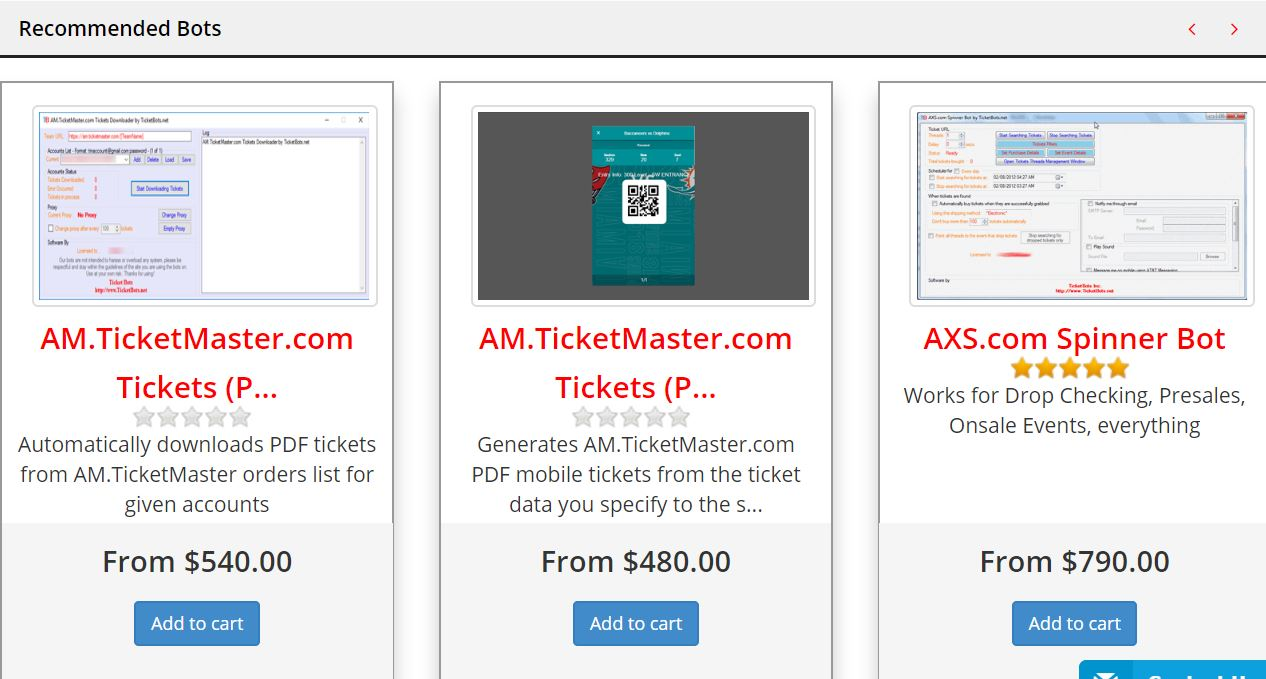
\includegraphics[width=0.68\textwidth]{chapter2/immagini/buybot}
	\caption{immagine presa dal sito \textit{ticketbots.net}}
	\label{buybot}
\end{figure}
Al momento non è ancora stata individuata, a livello software, una soluzione in grado di contrastare definitivamente l'attività di programmi che impersonano utenti "reali" e riescono a superare le prove poste dai siti di vendita, come ad esempio i cosiddetti "CAPTCHA" . Sono stati provati diversi approcci, che verranno descritti nel capitolo successivo. \`E stato dimostrato che, pur non esistendo al momento una concreta soluzione al problema, è possibile arginare in maniera parziale il problema dei "bot" tramite una combinazione di provvedimenti strategici e informatici, insieme alla collaborazione degli utenti. 
Recenti risultati mostrano che provvedimenti di tipo strategico, come modifiche al modello di vendita dei biglietti e delle politiche di pricing, hanno ottenuto risultati migliori nella lotta al Secondary Ticketing, in confronto alle leggi entrate in vigore negli ultimi vent'anni. 
Tale risultato può essere spiegato additando come ragione la mancanza di leggi con validità sovranazionale e con la scarso interesse delle autorità a combattere il fenomeno di rivendita \cite{drayer2011examining}.
\subsection{Architetture software dei portali di Secondary Ticketing}
Al momento, data la natura privata delle società che si occupano della gestione dei portali di Secondary Ticketing, non è possibile stabilire con certezza di quali meccanismi esse si avvalgano per l'acquisizione massiva di titoli di accesso e la gestione tecnologica dei portali accessibili tramite internet: non si conoscono infatti, ad esempio, le architetture software che gestiscono la vendita dei biglietti e i meccanismi di raccomandazione e promozione del portale. \'E possibile però avere un'idea generale di un portale di Secondary Ticketing grazie a un brevetto depositato nel 2002 da Brett Nakfoor alla Camera di Commercio statunitense \cite{nakfoor2002electronic}: tale invenzione descrive nei dettagli la creazione di un portale funzionante attivo sul mercato secondario. 
A livello di server, il sistema presenta una distinzione tra \textit{Database Server}, rappresentante la/le base/i di dati del portale, e \textit{Application Server}, sui quali risiede l'applicazione vera e propria. Il sistema si avvale inoltre di un router e di un firewall, in grado rispettivamente di smistare i messaggi da e verso l'applicazione e di filtrarli quando questi arrivano dal "mondo esterno", ovvero Internet. Un diagramma dell'architettura dei server è mostrato in Figura \ref{server}:
\begin{figure}[htbp]
	\centering
	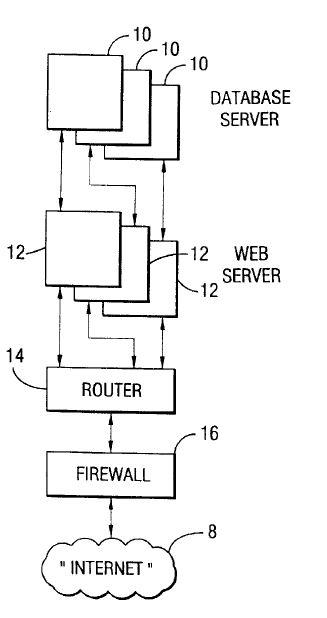
\includegraphics[width=0.68\textwidth]{chapter2/immagini/brevetto_app}
	\caption{Diagramma dell'architettura dell'applicazione lato server}
	\label{server}
\end{figure}
Il brevetto modellizza anche le interazioni tra mercato primario e secondario: ogni biglietto acquistato da canali ufficiali potrà essere messo in vendita sui portali secondari al prezzo desiderato con la modalità di pagamento preferita, ad esempio asta o vendita diretta, come mostra la Figura \ref{mercati}:
\begin{figure}[htbp]
	\centering
	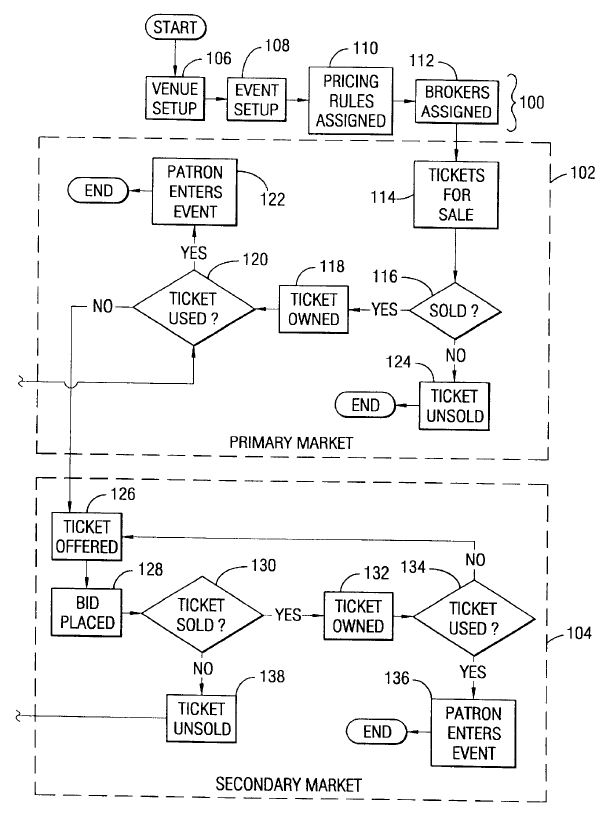
\includegraphics[width=0.68\textwidth]{chapter2/immagini/brevetto1}
	\caption{Diagramma dell'interazione tra mercato primario e secondario}
	\label{mercati}
\end{figure}
Come è possibile evincere dal diagramma, i biglietti non venduti sul mercato primario restano invenduti e non potranno essere rimessi in vendita, mentre tutti gli altri possono essere usati dal primo acquirente o essere rivenduti. Anche nel mercato secondario esiste la possibilità che un biglietto resti invenduto, magari per un prezzo eccessivo o per un errore nella stima della domanda da parte degli speculatori (broker) \cite{connolly2006rockonomics}.
\subsection{Differenze dagli altri mercati secondari}
Nel corso degli anni sono nate diverse piattaforme adibite al mercato secondario, in cui ogni utente può rimettere in vendita al prezzo desiderato un bene di proprietà: si pensi, ad esempio, a eBay, al marketplace di Facebook, a Craigslist, alla vendita di capi d'abbigliamento di lusso (es. StockX o Stadium Goods), o ai portali dedicati alla vendita di mezzi di trasporto, come auto e motocicli (es. Autoscout24).
Il mercato secondario dei titoli di accesso (biglietti) presenta però differenze sostanziali con gli altri marketplace: i biglietti sono infatti dei \textit{"perishable goods"} \cite{}, ovvero dei beni il cui valore presenta un alto valore di volatilità: a differenza di altri tipi di oggetto, come ad esempio un gioiello, un mezzo di trasporto o un capo di abbigliamento, il valore del biglietto è limitato nel tempo. Una volta emesso, il ticket avrà una validità fino al giorno dell'evento, dopodiché il suo valore sarà uguale a 0: per questo motivo è necessario porre particolare attenzione sul problema del \textit{pricing} sia nel mercato primario che quello secondario per mettere in evidenza le differenze e i parallelismi tra le differenti politiche attuate dagli attori coinvolti, come verrà infatti discusso nelle sezioni \ref{price} e \ref{dtp}. 

\section{Possibili cause del Secondary Ticketing}

\subsection{Funzioni di costo e avversità al rischio}
Diverse sono state le interpretazioni, nella storia, riguardanti le origini del fenomeno. Nel 1999, James Swofford mostrava le differenze sostanziali nelle funzioni di costo del rivenditore e dello speculatore: particolare attenzione è rivolta alle differenze nella concezione di Rischio e Incertezza tra speculatore e azienda produttrice \cite{swofford1999arbitrage}. 
La maggiore avversione al rischio dell'organizzatore, unita al desiderio di maggiori vendite e alla volontà di lucrare sulla vendita dei beni secondari, porta a una politica di "pricing" poco aggressiva: si tende, infatti, a tenere il prezzo dei titoli d'accesso più basso rispetto al reale valore di mercato. 
Un evento oggetto di grande attenzione pubblica, come ad esempio un tour negli stadi o nelle maggiori arene, o una finale di una particolare manifestazione sportiva, se il prezzo è troppo basso rispetto al valore di mercato, genera una domanda eccessiva e massicci fenomeni di rivendita: da una discordanza troppo elevata tra valore di mercato e di emissione può beneficiare lo speculatore, che ha la possibilità, spesso tramite avanzati software, di acquisire centinaia di titoli in pochi secondi. 
Swofford teorizza che per l'azienda il massimo profitto sia espresso dalla seguente equazione:
\begin{align*}
 \textbf{$max(P) = R(Q^{S})  - C(Q^{P})$}
\end{align*}
dove la funzione di guadagno R dipende dalle vendite, mentre la funzione di costo C rappresenta i costi sostenuti.
Lo speculatore ha una funzione di costo strettamente minore di quella del produttore, in quanto non sostiene i costi di produzione e di promozione. Si può così definire una seconda equazione che rappresenta il massimo profitto per lo speculatore ("scalper"): 
\begin{align*}
\textbf{$max(P) = R(Q^{S})  - C^{*}(Q^{P})$}
\end{align*}
Swofford teorizza che la funzione di costo dello speculatore sia strettamente minore di quella del promoter ($C^{*}(Q^{P}) < C(Q^{P}))$ per una serie di ragioni di ordine giuridico e tecnico:
\begin{itemize}
\item Lo speculatore non sostiene alcun costo di produzione, in quanto non è coinvolto in nessuna attività di organizzazione.
\item Lo speculatore ha meno costi di transazione e meno tasse da sostenere.
\item Lo speculatore spesso dispone di una vasta gamma di informazioni riguardanti l'evento, il possibile pubblico locale e relative disponibilità economiche.
\item Lo speculatore non risente di una eventuale cancellazione dell'evento, in quanto le vendite sul mercato secondario sono definitive, e inoltre non è coinvolto in alcuna spesa per gestire l'imprevisto.
\end{itemize}
La minore avversità al rischio da parte dello speculatore, unita ai minori costi da sostenere e alla capacità di accaparrarsi biglietti per spettacoli altamente richiesti, lo porta ad avere un mercato secondario di grosse dimensioni, che colpisce determinate tipologie di clienti.
Pascal Courty \cite{courty2003some} divide i fan in due categorie: 
\begin{itemize}
	\item \textbf{"Diehard fans"}, ovvero coloro che preferiscono comprare al momento dell'emissione dei biglietti, caratterizzati da un maggiore attaccamento nei confronti del performer e da minori liquidità. Questo dettaglio li porta a pianificare con attenzione e anticipo la propria partecipazione. 
	\item \textbf{"Busy Professionals"}, che non hanno la possibilità di pianificare con largo anticipo causa impegni di varia natura, e pertanto tendono ad acquistare in un secondo momento ("late market") . Tendenzialmente i secondi dispongono di più liquidità da investire rispetto ai primi e sono meno restii ad acquistare da agenti secondari, nel caso la reperibilità dei biglietti sul mercato primario venisse meno.
\end{itemize}

L'impossibilità di pianificare in dettaglio la propria presenza, insieme alla maggiore disponibilità economica, permette agli speculatori di incassare tutto il cosiddetto "\textit{Consumer Surplus}", ovvero la differenza tra la cifra che si è disposti a spendere e il valore effettivo del bene acquistato ("Face Value"). Il Consumer Surplus rappresenta l'oggetto del desiderio degli speculatori, che hanno interesse a redirigere verso di sé la quota di mercato che i rivenditori primari non riescono ad accaparrarsi. 
Courty teorizza che la vendita dei titoli di accesso sul mercato secondario avvenga a causa di intermediari che fanno da tramite tra il consumatore finale e il promoter, secondo lo schema illustrato in Figura \ref{st}: 
%Inserire immagine flusso bagarinaggio
\begin{figure}[htbp]
	\centering
	\includegraphics[width=0.68\textwidth]{chapter2/immagini/SchemaST}
	\caption{Rappresentazione della compravendita di titoli di accesso}
	\label{st}
\end{figure}
In aggiunta ai differenti interessi finanziari e speculativi, spesso la libera proliferazione del Secondary Ticketing è dovuta a una mancanza totale (o quasi) di regolamentazione normativa. Ergendo ad esempio il caso degli Stati Uniti, si nota che non tutti gli stati hanno regolamentazioni a riguardo, oppure si attengono ad emendamenti obsoleti risalenti agli anni '80, che non tengono conto dei progressi tecnologici e della posizione assunta dal mercato secondario nel corso degli anni \cite{courty2017ticket, drayer2011examining}.
La vasta presenza sul web di siti di Secondary Ticketing e la mancanza di una normativa federale unica fa sì che non sia possibile stabilire la giurisdizione di qualsiasi transazione avvenga su una piattaforma online.  
Emendamenti recenti hanno accentuato la tendenza alla "deregolamentazione" del mercato secondario, fedeli alla teoria del libero mercato di interscambio tra privati. è di particolare interesse il fatto che molte aziende adibite al commercio primario di titoli di accesso si siano dichiarate favorevoli a questa moda e abbiano addirittura incentivato lo sviluppo del mercato: su tutte spiccano Ticketmaster, titolare di diversi portali di rivendita, e molti club appartenenti alle maggiori leghe sportive statiunitensi (MLB, NFL, NHL, NBA), che possiedono portali dedicati su siti come StubHub e ViaGogo, nati in seguito ad accordi di natura commerciale tra le parti \cite{courty2014pricing}.
Le collaborazioni tra questi due enti stanno portando sempre di più a una totale legittimazione del mercato, poiché il mercato secondario ora gode di pieno appoggio, in cambio di una parte dei profitti, degli enti di rivendita primaria. Se da una parte una simile partnership riduce i rischi di contraffazione e di truffa nei confronti del consumatore, dall'altra mira a eliminare le differenze tra mercato primario e secondario, concependo la rivendita come una diretta conseguenza della vendita primaria. 

\subsection{Riallocazione efficiente dei biglietti}
Diversi ricercatori, tra cui Leslie, Sorensen \cite{leslie2013resale} e Karp \cite{karp2005promoters} sostengono che l'esistenza di un mercato secondario senza restrizioni porti verso una "riallocazione efficiente" dei biglietti, ovvero i titoli di accesso più ricercati e desiderati vengono assegnati al consumatore disposto a investire una maggiore quantità di denaro rispetto agli altri (ovvero gli utenti che hanno una maggiore \textit{Willingness to Pay}, o WTP) e non sono riusciti ad acquistare il biglietto in tempo utile sul mercato primario a causa di diversi fattori. Leslie e Sorensen infatti considerano il tempo come un importante fattore nella determinazione degli agenti che saranno in grado di acquistare sul mercato primario nel periodo delle vendite: viene definita infatti una funzione $C(t, \theta)$ (si ipotizza $C(t, \theta) \geq{0} $), decrescente in $t$ e crescente in $\theta$, che simboleggia lo sforzo (non necessariamente quantificabile in termini monetari) che comporta per un utente acquistare un biglietto il prima possibile (in termini di tempo e impegni personali, ad esempio). Si stima inoltre che per il consumatore finale il surplus generato dall'acquisto di un titolo di accesso di qualità $v$ e prezzo $p$ sul mercato primario sia uguale a: 
\begin{equation}
	U(v, \omega) - p - C(t, \theta)
\end{equation}
Per chi acquista da rivenditori non autorizzati invece l'utilità è data da: 
\begin{equation}
	r - p - C(t, \theta) - \tau
\end{equation}
Tale quantità, nel caso si decidesse di acquistare tramite rivenditori secondari, è con buona probabilità destinata a diminuire, poiché il prezzo di rivendita $r$ tende ad essere maggiore di $p$, spesso anche più del 30\%. Vanno inoltre considerati gli alti costi di transazione che l'utente sostiene ($\tau$). Sebbene quindi da una parte , l'esistenza di un mercato secondario dia la possibilità di acquistare i biglietti per i posti di maggiore qualità a coloro che hanno più liquidità da destinare all'acquisto, dall'altra viene irrimediabilmente danneggiato il consumatore interessato a partecipare all'evento, poiché godrà di meno benefici economici dall'acquisto. 

\subsection{Politiche di Pricing} \label{price}
Un argomento spesso dibattuto in letteratura è stato quello delle politiche di \textit{"pricing"} dei titoli di accesso (\cite{courty2012impact, bhave2017primary, esteves2009price, courty2011unpriced}). La scelta dei prezzi dei biglietti è un passaggio fondamentale nella lotta al bagarinaggio, ed è stato più volte notato che una cattiva scelta dei prezzi e una mancata valorizzazione della qualità dei posti della venue comporta copiosi fenomeni di Secondary Ticketing sui portali dedicati, in quanto è lì che il consumatore può effettivamente acquistare un posto della qualità desiderata al suo valore reale. In questa sezione verranno discussi due fenomeni, annoverati tra le principale cause del successo del Secondary Ticketing: il cosiddetto "\textit{Underpricing}" e la differenziazione dei prezzi in base alla loro qualità (\textit{Price Discrimination}).

\subsubsection{Underpricing}
La scelta di tenere i prezzi più bassi possibile può essere ricondotta a diverse logiche interne di business, ma anche alla volontà dell'artista coinvolto: 
\begin{itemize}
\item Dovendo un promoter sostenere molte spese prima dell'inizio dell'evento, come la prenotazione dello spettacolo desiderato, l'affitto della venue, contratti di fornitura e spese del personale, non è ammissibile correre il rischio di assegnare ai biglietti un valore maggiore del cosiddetto "market-clearing value", ovvero il prezzo ideale che riempirebbe esattamente la venue, senza lasciare domanda in eccesso non soddisfatta. La soluzione più intuitiva e meno rischiosa è pertanto quella di dare ai biglietti un prezzo minore del loro valore reale, con conseguenti fenomeni di speculazione. 
\item Il promoter non trae molti profitti dalle vendite dei biglietti (si parla di un guadagno medio intorno al 10/15\% dell'incasso totale), ma guadagna invece delle commissioni sulla vendita del merchandising, oltre che una percentuale su servizi complementari come la vendita di cibo e il parcheggio. Limitare i prezzi dei biglietti garantisce una maggiore possibilità di trarre profitti dalle vendite di beni secondari, che per il promoter rappresentano gran parte dell'incasso (revenue).
\item L'artista tiene a mantenere un rapporto di lealtà coi fan e, per una questione di immagine, cerca di non apparire come approfittatore. Sempre per quanto riguarda il punto di vista dell'artista, un prezzo contenuto del biglietto permette al fan/partecipante di acquistare merchandising, sul quale l'artista (e/o il suo staff) trattiene gran parte dei guadagni. Si stima che gli artisti trattengano una percentuale tra l'80 e il 90\% delle vendite dei biglietti \cite{phdthesis, tompkins2018ticket}. 
\item \'E importante considerare come fattore determinante del successo di un evento la felicità di chi vi ha preso parte. Se un partecipante ha tratto un'esperienza positiva dall'evento, è possibile che in futuro si rechi con maggiore probabilità a eventi organizzati dello stesso promoter, o che torni presso la stessa venue. Si cerca quindi di costruire un rapporto di lealtà tramite un processo di fidelizzazione (\cite{tompkins2018ticket}).
\end{itemize}
Questa politica spesso però non tiene conto del reale valore dei biglietti e di quanto il partecipante possa realmente essere disposto a investire pur di prendere parte all'evento. Non è raro infatti vedere biglietti rivenduti sul mercato secondario con ricarichi (\textit{markup}) anche superiori al 60\%. Per i posti migliori capita inoltre che alcuni titoli vengano rivenduti a prezzi anche superiori al 500\% del valore originale. A supporto di quanto indicato, vengono ora mostrate delle immagini raffiguranti i prezzi, su mercato primario e secondario, della data del tour di Vasco Rossi, schedulata per il 1/06/2019 presso lo stadio San Siro di Milano (screenshot effettuati in data 22/03/2019): 
\begin{figure}[H]
    \centering
    \begin{minipage}{0.45\textwidth}
        \centering
        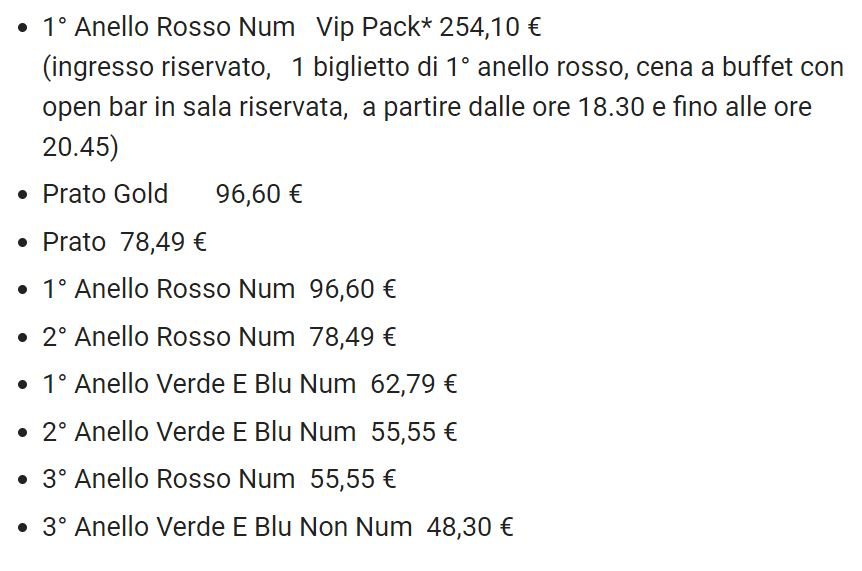
\includegraphics[width=0.9\textwidth]{chapter2/immagini/vascofv} % first figure itself
        \caption{Prezzi dei canali ufficiali (Vivaticket)}
    \end{minipage}\hfill
    \begin{minipage}{0.45\textwidth}
        \centering
        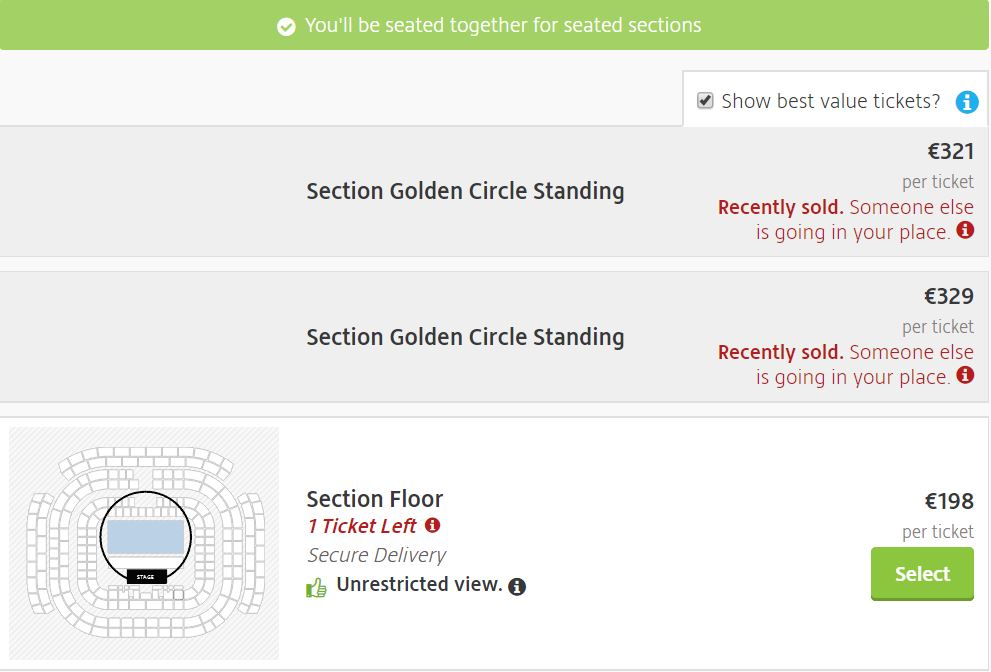
\includegraphics[width=0.9\textwidth]{chapter2/immagini/vascost} % second figure itself
        \caption{Prezzi su Viagogo per le posizioni Prato e Prato Gold}
    \end{minipage}
\end{figure}

\subsubsection{Price Discrimination}
Un'altra causa del successo del Secondary Ticketing è sicuramente la scarsa considerazione della diversa qualità dei posti di ogni venue. La tendenza, per la gran parte dei concerti di musica leggera, è quella di emettere biglietti tutti allo stesso prezzo, senza tenere conto delle effettive differenze: si stima che mediamente più del 70\% dei concerti usino questo approccio \cite{leslie2013resale, esteves2009price}. L'adozione di una logica che non consideri l'effettiva qualità dei posti (es. vicinanza al palco, lateralità ecc.) fa sì che buona parte del consumer surplus che non è catturata nella prima fase di vendita venga poi catturata dai rivenditori e dagli speculatori, che invece scelgono di rivendere a prezzi maggiorati anche in base alla qualità percepita del posto e all'interesse della comunità. 
Si stima che mediamente i concerti prezzati con politiche efficienti di Price Discrimination abbiano ritorni economici mediamente maggiori del 5\% rispetto agli eventi in cui tutti i titoli d'accesso hanno prezzo unico \cite{courty2012impact}. Tale risultato si spiega con il fatto che, con una simile politica di allocazione dei biglietti, i consumatori con maggiore disponibilità economica e interesse per la qualità del posto scelgano i posti per loro allocati, generalmente più costosi e in posizioni migliori, in termini di visibilità e qualità del suono. %\subsection{Mancanza di trasparenza nell'allocazione dei biglietti}

\section{Impatti del Secondary Ticketing sugli Stakeholder}
La ricercatrice Mielko nel corso del 2017 ha mostrato che gli impatti del Secondary Ticketing non si limitano soltanto ai consumatori finali, ovvero coloro che prenderanno parte alla manifestazione desiderata, ma danneggiano promoter, artisti e il luogo dell'evento ("\textit{Venue}").
\subsection{Danni per il Promoter}
Come dimostrato da Swofford, Courty e Tompkins, il promoter propende verso una politica di "underpricing" dei titoli di accesso rispetto al reale valore di mercato. I motivi di maggiore rilevanza sono sotto elencati: 
\begin{itemize}
\item Si vuole garantire al consumatore un "surplus" consistente, che garantisca soddisfazione e lasci una liquidità da spendere il giorno dell'evento per i "beni secondari"
\item La messa in vendita di biglietti a un prezzo percepito come troppo elevato è rischiosa in quanto le vendite potrebbero non essere sufficienti a coprire i costi sostenuti e potrebbero compromettere l'effettivo svolgimento dell'evento. 
\item Il promoter guadagna anche in base alle percentuali sulle vendite di merchandising, parcheggi e "beni secondari", pertanto è fondamentale che il consumatore finale non si senta "derubato" ("price gouging").
\item Si vuole costruire un rapporto di lealtà e fidelizzazione coi propri clienti, in modo da poter costruire un rapporto di collaborazione a lungo termine.
\end{itemize}
\subsubsection{Danni economici}
Se da una parte il fenomeno del Secondary Ticketing funge da mitigatore di rischio \cite{geloso2014ticket} per il consumatore e provvede alla corretta riallocazione dei biglietti invenduti (o rivenduti) in base al loro vero valore di mercato e alla disponibilità economica (\textit{willingness to pay}) del consumatore, dall'altra genera problematiche riguardo all'evento coinvolto: i guadagni derivanti dalla rivendita infatti non sono in alcun modo destinati al promoter, e spesso addirittura non viene corrisposta neanche una commissione al fisco del paese di riferimento, in quanto molte vendite avvengono sul mercato nero. 
Un errore nel pricing iniziale del biglietto può costare caro al promoter responsabile dello svolgimento corretto della manifestazione, poiché si perde ogni forma di tracciabilità dei titoli di accesso commerciati sul mercato secondario: un tale fenomeno rende impossibile e quasi impraticabile la stima esatta dei partecipanti e le stime dei costi da sostenere.
\subsubsection{Danni reputazionali}
Un altro problema derivante dalla vendita sul mercato secondario è l'impossibilità, per un promoter, di stabilire con precisione l'identità dei partecipanti all'evento organizzato e, di conseguenza, l'incapacità di stabilire una relazione solida e di fiducia con potenziali clienti futuri: non sarà infatti possibile organizzare e direzionare in maniera efficiente campagne promozionali di marketing a un grosso gruppo di persone, fallendo così ogni tentativo di sensibilizzazione.
Cresce inoltre il rischio che i dati delle presenze il giorno della manifestazione non corrispondano a quelli delle vendite, perché grosse quantità di titoli d'accesso restano invendute, danneggiando l'immagine del "performer".  
\subsubsection{Mancanza di controlli sulla distribuzione dei biglietti}
Una importante questione sulla quale l'opinione pubblica ha da tempo cercato di sensibilizzare è la modalità di vendita dei biglietti, con un focus particolare sulle quantità reali messe in vendita.
Si stima che, per quanto concerne gli eventi di grande portata, una cospicua porzione dei posti migliori venga riservata ancora prima della messa in vendita dei biglietti: si tratta degli ingressi riservati ("`o biglietti di cortesia"') a management, amici e parenti degli artisti, stampa e personalità di spicco. Unita alla porzione di biglietti riservata alle prevendite (es. possessori di una data carta o credito o membri di un dato fan club), Tompkins \cite{tompkins2018ticket} nota che spesso al pubblico vero e proprio vengono messi a disposizione meno del 50\% della capienza della venue. Una simile disposizione dei titoli di accesso altera il mercato dell'evento e dà luogo a consistenti fenomeno di Secondary Ticketing, in quanto non rispecchia il reale dato sulle vendite e non riflette il reale interesse sull'evento, ma è soltanto un mezzo per fingere il "sold out" e recuperare parte dei costi di inventario tramite la vendita di beni secondari.  
 
\subsection{Danni per il consumatore}
Il consumatore è da considerarsi parte lesa in quanto risulta danneggiato: 
\begin{itemize}
\item Dal punto di vista economico, in quanto risente sia del rincaro del mercato secondario che di quello primario, che tende ad alzare i listini come risposta agli speculatori. Questo porta a ridurre il numero medio di concerti frequentati mediamente dal singolo consumatore \cite{eckard2013impact}.
\item Dal punto di vista della soddisfazione, Il surplus diminuisce notevolmente in seguito all'aumento dei prezzi e al proliferare delle soluzioni di mercato secondario. Anzi, tali eventi possono anche portare all'esclusione di una data fascia di consumatori da una serie di eventi ai quali prima avrebbero potuto prendere parte con la loro disponibilità economica \cite{perez2016music}, mentre ora rischiano di non poterselo più permettere.
\item Psicologicamente, in quanto prova sentimenti di frustrazione in seguito all'incapacità di acquistare il biglietto desiderato al prezzo di emissione. 
\end{itemize}

\subsection{Danni per l'artista}
L'artista coinvolto nella manifestazione non è esente da danni economici e reputazionali causati dal Secondary Ticketing. Tompkins  \cite{tompkins2018ticket} mostra che gli artisti incassano una percentuale delle vendite dei biglietti che si aggira tra l'85\% e il 90\%, ma non possono in alcun modo trarre proventi dalle vendite sul mercato secondario: pertanto si vedono sfuggire una grossa quota di mercato, "catturata" da un piccolo gruppo di speculatori. In aggiunta, è stato notato che, in eventi colpiti in maniera massiva dal fenomeno del mercato secondario, i fan sono più restii a spendere in beni secondari come bevande e merchandising, su cui l'artista guadagna una percentuale. Inoltre, spesso la reputazione dell'artista viene lesa quando grandi quantità di utenti acquistano da portali di rivendita, in quanto spesso il consumatore non è in grado di riconoscere tali siti, ed è convinto si tratti di una semplice vendita primaria. 
\'E compito dell'artista inoltre assicurarsi di costruire un rapporto di fedeltà e lealtà coi propri fan, motivo per cui serve discostarsi il più possibile dal mercato secondario ed eventuali accuse di speculazione. 

\section{Esempi concreti di Secondary Ticketing}
Nella storia sono riscontrabili numerosi episodi, spesso di rilevanza internazionale, di Secondary Ticketing. Ne verranno discussi alcuni tra i più recenti e rilevanti in ordine cronologico.
\'E interessante notare come, nei casi descritti, i provvedimenti maggiori siano stati intrapresi dagli artisti, mentre i rivenditori autorizzati primari spesso hanno cercato di minimizzare il problema giustificandolo con un'eccessiva richiesta di titoli di accesso \cite{fortunato2011dancing}.
 
\subsection{2009: Springsteen contro Ticketmaster}
Nel 2009, Bruce Springsteen annunciava il "\textit{Working on a Dream Tour}", programmato per la primavera nei maggiori palazzetti degli Stati Uniti. In seguito a un'indagine federale emerse che Ticketmaster, rivenditore autorizzato con esclusiva, in occasione della vendita delle uniche due date nello stato del New Jersey, aveva automaticamente reindirizzato un numero indefinito di clienti (circa mille per data, stando alle indagini federali) sul proprio portale di Secondary Ticketing \textit{TicketsNow} a prezzi notevolmente maggiorati, senza avvisare in alcun modo gli utenti. TicketsNow fu inoltre indagato per aver venduto centinaia di biglietti contraffatti o inesistenti a prezzi inflazionati. \\
TicketMaster non ammise mai le responsabilità, e rispose alle accuse solo in seguito all'apertura dell'inchiesta: pagò inoltre circa 350000\$ di spese legali. Successivamente fu inoltre invitata a fornire accesso alle proprie tecnologie in modo da permettere a nuovi concorrenti nel mondo del ticketing di emergere (come ad esempio AEG, \cite{fortunato2011dancing})

\subsection{2012: "Shameless Sandy Outrage"}
Il concerto di beneficienza, tenutosi il 12/12/12 a New York, US, fu ai tempi oggetto di grande attenzione mediatica: l'evento, svoltosi al Madison Square Garden, contava, tra gli altri, ospiti come Bruce Springsteen, Kanye West, Eddie Vedder, Billy Joel e Paul McCartney, ed il suo svolgimento era funzionale a una raccolta fondi in sostegno delle vittime dell'uragano Sandy del 2012.
Da un'analisi del New York Post emerse che molti biglietti erano stati venduti sulla piattaforma secondaria StubHub (eBay), con un ricarico medio del 273\%, mentre altri 900 biglietti erano ancora in vendita su portali secondari. Stando ai dati forniti da StubHub, il biglietto più costoso fu venduto per la cifra di 3700 dollari, contro i 2500 del valore di emissione. 
L'evento suscitò scalpore in quanto fu un caso rilevante di uso massivo dei "ticket BOT", avanzati software in grado di acquistare centinaia di biglietti al minuto, in maniera nettamente più rapida di un essere umano. (\$uperscalp Sandy outrage, New York Post, 7/12/2012, \cite{tompkins2018ticket})

\subsection{2016: caso Chance the Rapper}
Nel settembre 2016, lo statiunitense \textit{Chance the Rapper} riacquista da Viagogo circa 2.000 biglietti, scegliendo di rimetterli in vendita al loro reale valore di emissione in forma cartacea, in modo da scoraggiare una seconda rivendita. 
\begin{figure}[htbp]
    \centering
    \begin{minipage}{0.45\textwidth}
        \centering
        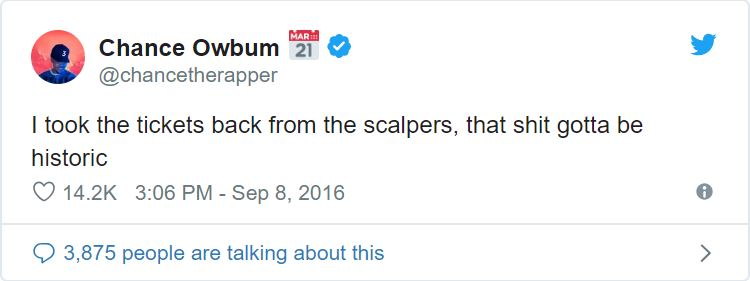
\includegraphics[width=0.9\textwidth]{chapter2/immagini/chance1} % first figure itself
        \caption{Primo tweet riguardante il fatto}
    \end{minipage}\hfill
    \begin{minipage}{0.45\textwidth}
        \centering
        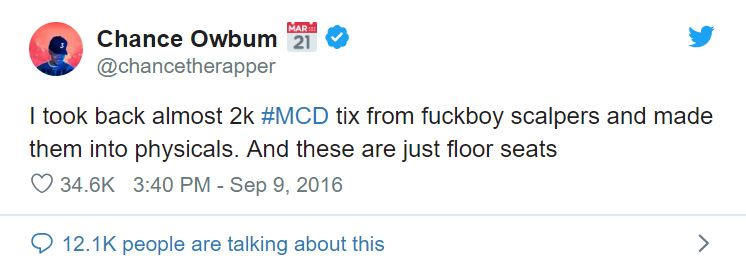
\includegraphics[width=0.9\textwidth]{chapter2/immagini/chance2} % second figure itself
        \caption{Secondo tweet}
    \end{minipage}
\end{figure}

\subsection{2016: caso Coldplay}
A ottobre 2016 la band inglese annunciava due date italiane per il luglio dell'anno successivo presso lo Stadio San Siro di Milano. Al momento della vendita, i biglietti durarono pochi secondi sulla piattaforma Ticketone prima di essere rivenduti su portali come Viagogo, eBay e Stubhub. Un caso simile dimostrò un'altra volta la totale incapacità dei sistemi informativi di e-commerce di prendere provvedimenti contro i bot automatizzati, se non l'inesistenza di una simile precauzione.
Venne aperta un'inchiesta con le accuse di agiotaggio e falsificazione di dati di mercato per gli amministratori delegati delle società coinvolte, conclusasi nel febbraio 2019 con l'assoluzione totale delle persone coinvolte (Corriere della Sera, 2019). 

\subsection{2018: Ed Sheeran collabora con Agenti Federali}
A cavallo tra il 2017 e il 2018, la popstar britannica Ed Sheeran ha collaborato con il National Trading Standards Cyber Crime team, un ristretto gruppo di agenti federali specializzati in frode informatica, allo scopo di tracciare i biglietti pervenuti sul mercato secondario. Tramite un'analisi dei pattern di compravendita della mole di biglietti, gli agenti hanno confiscato circa 25.000 biglietti a Viagogo, per poi rimetterli in vendita sul circuito primario. \\
Al momento, questa operazione di analisi del trend degli acquisti sui portali primari di vendita è stata una delle poche in grado di riuscire a riconoscere dei pattern di acquisto tipici dei bot. 
Se da una parte una tale scoperta rappresenta un passo avanti nella lotta al Secondary Ticketing, dall'altra mostra anche le carenze, dal punto di vista tecnico, nel riconoscimento preventivo di agenti di acquisto automatizzati: non è ancora possibile, anche tramite complessi firewall, impedire l'accesso alle vendite ai bot, in quanto ai sistemi gli acquisti risultano effettuati da utenti regolari. 